\documentclass[compress]{beamer}

\usepackage[nofonts]{ctex}
\setCJKmainfont[ItalicFont={Kaiti SC}]{Kaiti SC}%
%\setCJKmainfont[ItalicFont={AR PL KaitiM GB}]{AR PL KaitiM GB}%
%\setCJKsansfont{WenQuanYi Zen Hei}% 文泉驿的黑体

\mode<beamer>
{
    \setbeamercovered{transparent}
    \useinnertheme{rounded}
    \useoutertheme{split}
    \usecolortheme{rose}
    \usecolortheme{seahorse}

	\expandafter\def\expandafter\insertshorttitle\expandafter{%
	\insertshorttitle\hfill%
	\insertframenumber\,/\,\inserttotalframenumber}
}

\mode<handout>
{
	\usetheme{default}
	\usepackage{pgfpages}
	\pgfpagesuselayout{4 on 1}[a4paper,landscape,border shrink=5mm]
}


\usepackage{amsmath,latexsym,amssymb,amsfonts,amsbsy}
\usepackage{graphicx}
\usepackage{hyperref}
\usepackage{fancyvrb}
\fvset{frame=single,tabsize=4, numbers=left, fontsize=\small}

\newcommand{\romannumber}[1]{{\textrm{\uppercase\expandafter{\romannumeral
#1}}}}
\setbeamercolor{dblue}{fg=white,bg=blue!40!black} % for beamercolorbox
\newenvironment{pblock}{\begin{beamercolorbox}[rounded=true,
               shadow=true]{dblue}}{\end{beamercolorbox}}

\graphicspath{{figure/}}

%%%%%%%%%%%%%%%%%%%%%%%%%%%%%%%%%%%%%%%%%%%%%%%%%%%%%%%%%%%%%%%%%
%    body                                                       %
%%%%%%%%%%%%%%%%%%%%%%%%%%%%%%%%%%%%%%%%%%%%%%%%%%%%%%%%%%%%%%%%%


\begin{document}

\AtBeginSection[]
{ 
    \begin{frame}<beamer> 
		\frametitle{内容提要} 
		\tableofcontents[currentsection,currentsubsection] 
	\end{frame} 
} 
					
\title{深入Makefile}

\author[\href{http://c.pku.edu.cn/}{http://c.pku.edu.cn/}]
{曹东刚\\\href{mailto:caodg@sei.pku.edu.cn}{caodg@sei.pku.edu.cn}}

\institute{Linux程序设计环境 \\
\href{http://c.pku.edu.cn/}{
http://c.pku.edu.cn/}}

\date{}

\titlegraphic{\includegraphics[height=0.17\textwidth]{Overlays/logo.pdf}}

\begin{frame}
	\titlepage
\end{frame}

\section{make高级技巧}


\subsection{规则}

\begin{frame}
\frametitle{makefile和源文件不在一个目录下}

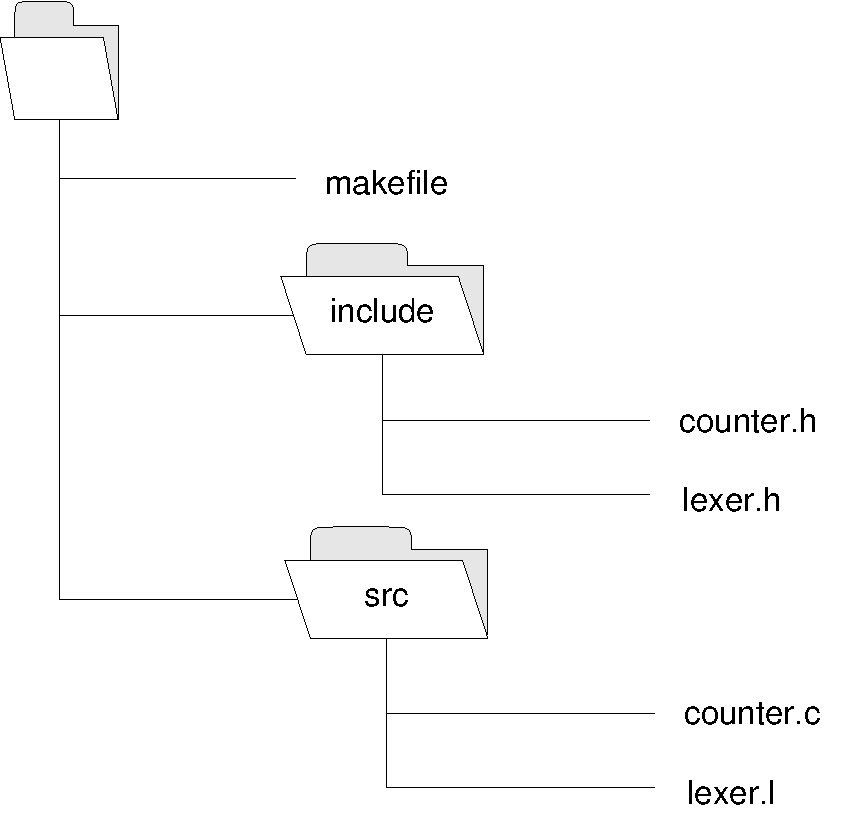
\includegraphics[width=0.7\hsize]{folder.pdf}


\end{frame}


\begin{frame}[containsverbatim]
\frametitle{VPATH和vpath}

\begin{Verbatim}
VPATH    = src include
CPPFLAGS = -I include

count_words: counter.o lexer.o -lfl
count_words.o: counter.h
counter.o: counter.h lexer.h
lexer.o: lexer.h
\end{Verbatim}

也可以使用命令:
\begin{Verbatim}
vpath %.c src
vpath %.h include
\end{Verbatim}

\end{frame}

\begin{frame}[containsverbatim]
\frametitle{内置的模式规则 --- 1}
从.c生成.o文件\\
\begin{Verbatim}[showtabs=true]
%.o:%.c
	$(COMPILE.c) $(OUTPUT_OPTION) $<
\end{Verbatim}
从.l生成.c文件\\
\begin{Verbatim}[showtabs=true]
%.c:%.l
	@$(RM) $@
	$(LEX.l) $< > $@
\end{Verbatim}

\end{frame}

\begin{frame}[containsverbatim]
\frametitle{内置的模式规则 --- 2}

从.c生成可执行文件\\
\begin{Verbatim}[showtabs=true]
%:%.c
	$(LINK.c) $^ $(LOADLIBES) $(LDLIBS) -o $@
\end{Verbatim}
\end{frame}

\begin{frame}[containsverbatim]
\frametitle{静态模式规则}

静态模式规则: 明确给出了目标列表\\
\begin{Verbatim}[showtabs=true]
$(OBJECTS):%.o:%.c
	$(CC) -c $(CFLAGS) $< -o $@
\end{Verbatim}

应当尽可能使用静态模式规则, 明确写出目标之间的依赖关系

\end{frame}

\begin{frame}[containsverbatim]
\frametitle{后缀规则}
后缀规则是定义隐式规则的初始方式.\\[1ex]
\begin{Verbatim}[showtabs=true]
.c.o:
    $(COMPILE.c) $(OUTPUT_OPTION) $<
\end{Verbatim}
等价于:
\begin{Verbatim}[showtabs=true]
%.o:%.c
    $(COMPILE.c) $(OUTPUT_OPTION) $<
\end{Verbatim}

\end{frame}

\begin{frame}[containsverbatim]
  \frametitle{单后缀规则}
单后缀规则常用于生成可执行文件 \\
\begin{Verbatim}[showtabs=true]
.p:
	$(LINK.p) $^ $(LOADLIBES) $(LDLIBS) -o $@
\end{Verbatim}
\end{frame}

\begin{frame}[containsverbatim]
\frametitle{内置规则的结构}

\begin{Verbatim}[showtabs=true]
%.o: %.c
	$(COMPILE.c) $(OUTPUT_OPTION) $<
\end{Verbatim}

变量:
\begin{Verbatim}[showtabs=true]
COMPILE.c = $(CC) $(CFLAGS) $(CPPFLAGS) \
	$(TARGET_ARCH) -c
CC = gcc
OUTPUT_OPTION = -o $@
\end{Verbatim}

\end{frame}

\begin{frame}[containsverbatim]
\frametitle{自动生成依赖}

问题: C语言源文件依赖头文件, 头文件之间也有依赖, 能否自动生成并管理这种
依赖? \\
方法: 利用gcc的编译选项\verb~gcc -M~ \\

\end{frame}


\begin{frame}[containsverbatim]
  \frametitle{gcc编译开关}
{\tiny
\begin{Verbatim}
~ $ echo "#include <stdio.h>" > stdio.c
~ $ gcc -M stdio.c
stdio.o: stdio.c /usr/include/stdio.h \
  /usr/include/_ansi.h \
  /usr/include/newlib.h \
  /usr/include/sys/config.h \
  /usr/include/machine/ieeefp.h \
  /usr/include/cygwin/config.h \
  /usr/lib/gcc/i686-pc-cygwin/3.4.4/include/stddef.h \
  /usr/lib/gcc/i686-pc-cygwin/3.4.4/include/stdarg.h \
  /usr/include/sys/reent.h \
  /usr/include/_ansi.h \
\end{Verbatim}
}

\end{frame}

\begin{frame}[containsverbatim]
\frametitle{方法}

\begin{itemize}
\item 为每个源文件(filename.c)生成一个依赖文件, 如filename.d
\item 该filename.d里面保存了filename.c和filename.d对头文件的依赖, 如: 
\begin{verbatim}
counter.o counter.d : src/counter.c \
	include/counter.h include/lexer.h
\end{verbatim}
\item 用包含命令(include)将所有filename.d包含在makefile中
\end{itemize}

\end{frame}

\begin{frame}[containsverbatim]
\frametitle{生成filename.d}
\begin{Verbatim}[showtabs=true]
include $(subst .c,.d,$(SOURCES))

%.d: %.c
	$(CC) -M $(CPPFLAGS) $< > $@.$$$$;          \
	sed 's/\($*\)\.o[ :]*/\1.o $@ : /g' < $@.$$$$ > $@; \
	rm -f $@.$$$$
\end{Verbatim}

\end{frame}

\subsection{变量}

\begin{frame}[containsverbatim]
\frametitle{make变量}

\begin{itemize}
\item make实际上包含两种语言: 描述依赖关系的语言, 以及进行文本替换的宏语言
\item 变量名字几乎可以是任何字符, 除了 \verb~: # =~
\item 变量大小写敏感
\item 变量可以通过 \verb~${CC}~或者\verb~$(CC)~访问
\end{itemize}
\end{frame}

\begin{frame}
\frametitle{make变量}

\begin{itemize}
\item 通常如果用户希望通过命令行或环境变量改变某变量的值, 则这样的常量名字全部大写, 单词之间通过下划线分隔
\item 全部小写的变量只用于makefile文件内部
\item 通常用变量引用外部程序名
\end{itemize}
\end{frame}

\begin{frame}[containsverbatim]
\frametitle{变量扩展}
\begin{itemize}
\item 简单扩展, 通过``\verb~:=~''赋值. 赋值语句被make读到的时候, 即对赋值符右侧进行扩展\\
\verb~MAKE_DEPEND := $(CC) -M~ \\
如果 CC没有定义, 则赋值的结果为: \verb*~ -~M
\item 递归扩展, 通过``\verb~=~''赋值. 只有当变量被make用到的时候, 才对赋值符右侧进行扩展\\
\verb~MAKE_DEPEND = $(CC) -M~ \\
CC 的定义可以在\verb~MAKE_DEPEND~的后面
\end{itemize}

\end{frame}

\begin{frame}[containsverbatim]
\frametitle{宏}

\begin{Verbatim}[showtabs=true]
define create-jar
 @echo Creating $@...
 $(RM) $(TMP_JAR_DIR)
 $(MKDIR) $(TMP_JAR_DIR)
 $(CP) -r  $^ $(TMP_JAR_DIR)
 cd $(TMP_JAR_DIR) && $(JAR) $(JARFLAGS) $@ .
 $(JAR) -ufm $@ $(MANIFEST)
 $(RM) $(TMP_JAR_DIR)
endef

$(UI_JAR): $(UI_CLASSES)
	$(create-jar)
\end{Verbatim}

\end{frame}

\begin{frame}
\frametitle{函数}
GNU make 支持函数\
\begin{itemize}
\item 函数的定义和宏的定义类似
\item 函数的调用和变量的引用类似, 只是要加上逗号分隔的参数列表
\end{itemize}

\end{frame}

\begin{frame}[containsverbatim]
\frametitle{用户自定义函数}


\begin{Verbatim}
# cygwin script
AWK  := awk
KILL := kill

# $(kill-acroread)
define kill-acroread
  @ ps -aw |                               \
  $(AWK) ' /AcroRd32/ {                    \
               print "Killing " $$3;       \
               system( "$(KILL) " $$1 )    \
           }'
endef
\end{Verbatim}

\end{frame}

\begin{frame}[containsverbatim]
\frametitle{用户自定义函数}

\begin{Verbatim}[showtabs=false]
AWK  := awk
KILL := kill
# $(call kill-program, awk-pattern)
define kill-program
	@ ps -aw |                       \
	$(AWK) ' /$1/ {                  \
		print "Killing " $$3;        \
		system( "$(KILL)  " $$1 )    \
	}'
endef
\end{Verbatim}

\noindent 调用: \verb~$(call kill-program, "AcroRd32")~

\end{frame}

\begin{frame}[containsverbatim]
\frametitle{内置函数}
GNU make有若干内置函数, 用于对变量进行操作.
函数使用语法: \verb~ $(function-name arg1[, argn])~
\begin{itemize}
\item 字符串操作函数
\item 文件名操作函数
\item 流程控制函数
\item 用户自定义函数
\item 其它函数
\end{itemize}
\end{frame}

\begin{frame}[containsverbatim]
\frametitle{字符串函数}
\verb~$(filter pattern...,text)~ , text: 空格分隔的单词串, 
  返回完整匹配的单词. 例:\\
{\small
\begin{Verbatim}[showtabs=true]
words := he the hen other the%
get-the:
	@echo %he matches : $(filter %he,$(words))
\end{Verbatim}
}

\verb~$(subst search-string,replace-string,text)~ , 将text中的search-string替换为replace-string. 例:\\
{\small
\begin{Verbatim}
sources := count_words.c counter.c lexer.c
objects := $(subst .c,.o,$(sources))
\end{Verbatim}
}
\end{frame}

\subsection{命令}

\begin{frame}[containsverbatim]
\frametitle{命令}

\begin{itemize}
\item 目标之后以制表键TAB开头的行为命令
\item 命令本质上是一个一行的shell脚本
\item makefile中的命令在子shell中执行
\item 命令执行的shell缺省是/bin/sh, 由make 的变量SHELL控制
\item make命令执行时继承父shell的除SHELL外的所有变量
\item 需要由shell扩展的参数应该用\verb~$$n~的形式
\end{itemize}
\end{frame}

\begin{frame}[containsverbatim]
\frametitle{命令解析}
make看到一个合法命令之后, 即转入命令解析模式, 建立一个一行脚本
\begin{itemize}
\item 以制表键缩进的行被认为是命令行
\item 空行被忽略
\item 以\verb~#~开始的行(之前可能有空格, 但没有制表键)被认为是makefile注释, 被忽略
\item 条件处理指令, 如 \alert{ifdef} 和 \alert{ifeq}在命令脚本中处理
\end{itemize}

\end{frame}

\begin{frame}[containsverbatim]
\frametitle{注释}
\begin{itemize}
\item makefile注释: 不在命令中的以\verb~#~开头(前面可有空格)的行, 被make忽略处理
\item shell注释: 在命令中, 以制表符加\verb~#~开头的行, make要对其进行扩展, 然后交给shell处理; 每个注释都会启动一个子shell
\end{itemize}
\end{frame}

\begin{frame}[containsverbatim]
  \frametitle{注释示例}

\begin{Verbatim}[showtabs=true]
#this is make comment $(PWD)
print-pwd:
	#
	# this is shell comment
	# PWD = $(PWD)
	# $(findstring /e/home/Make,$(PWD))
	#
\end{Verbatim}
\end{frame}

\begin{frame}[containsverbatim]
\frametitle{长命令}
由于每个命令在单独的一个子shell中执行, 如果若干命令要在一起执行, 需要用反斜杠\verb~\~连接各行\\

例: 错误的写法
\begin{Verbatim}[showtabs=true]
filie_list:
	for f in logic ui
	do
		echo $f/*.java
	done > $@
\end{Verbatim}
\end{frame}

\begin{frame}[containsverbatim]
\frametitle{长命令}
正确的写法
\begin{Verbatim}[showtabs=true]
filie_list:
	for f in logic ui; \
	do \
		echo $$f/*.java; \
	done > $@
\end{Verbatim}
\end{frame}

\section{生成Makefile}

\subsection{动机}

\begin{frame}
\frametitle{为什么要自动生成Makefile}
\begin{itemize}
  \item 可移植性: 适应不同硬件平台和Unix系统
	\begin{itemize}
	  \item 机器字大小、工具、语言、服务器、设置等
		\begin{itemize}
		  \item 例如, bcopy与memcpy
		\end{itemize}
	\end{itemize}
  \item 派生依赖性: C语言源文件之间的依赖关系
\end{itemize}
\end{frame}

\begin{frame}
  \frametitle{几种主要生成工具}
  \begin{itemize}
	\item \alert{makedepend}
	\item Imake
	\item \alert{autoconf}
	\item automake
  \end{itemize}
  
\end{frame}

\begin{frame}[containsverbatim]
  \frametitle{makedepend}
  \begin{itemize}
	\item 随X Window系统发布
	\item 在解决源码依赖方面最快, 最有效
	\item 只对C项目, 分析C源文件的\verb~#include~等宏指令
	\item 将依赖关系生成到Makefile中
  \end{itemize}
  
\end{frame}

\begin{frame}[containsverbatim]
  \frametitle{makedepend示例}
  通常将makedepend作为Makefile的一个目标通过make调用\\
\begin{Verbatim}[showtabs=true]
SRCS = Main.c Print.c

all: print
print: Main.o Print.o
	gcc -o $@ $^

depend:
	makedepend ${SRCS}
\end{Verbatim}
\end{frame}

\begin{frame}[containsverbatim]
  \frametitle{makedepend更新后的Makefile}
\begin{Verbatim}[showtabs=true,fontsize=\footnotesize]
SRCS = Main.c Print.c
all: print
print: Main.o Print.o
	gcc -o $@ $^
depend:
	makedepend $(SRCS)
# DO NOT DELETE
Main.o: Print.h
Print.o: /usr/include/stdio.h /usr/include/features.h
Print.o: /usr/include/sys/cdefs.h /usr/include/gnu/stubs.h
Print.o: /usr/lib/gcc-lib/i486-linux/3.3.5/include/stddef.h
Print.o: /usr/include/bits/types.h /usr/include/bits/wordsize.h
Print.o: /usr/include/bits/wchar.h /usr/include/gconv.h
Print.o: Print.h
\end{Verbatim}
  
\end{frame}

\subsection{autoconf}

\begin{frame}
  \frametitle{autoconf}
  GNU项目发布约定
  \begin{itemize}
	\item 编译过程分两个步骤: 产生编译配置、编译
	\item 项目根目录下有一个\alert{configure}脚本, 用于生成Makefile
	\item configure读取\alert{Makefile.in}文件, 生成Makefile及其他可能辅助的文件
	\item 调用标准的make进行编译
  \end{itemize}
  
\end{frame}

\begin{frame}
  \frametitle{autoconf支持的项目目录结构}
\begin{itemize}
  \item flat: 所有文件都位于同一个目录中, 且没有子目录
	\begin{itemize}
	  \item 最简单
	\end{itemize}

  \item shallow: 源代码都储存在顶层目录,其他各个部分则储存在子目录中
  \item deep: 所有源代码都被储存在子目录中;顶层目录主要包含配置信息
	\begin{itemize}
	  \item 最复杂
	\end{itemize}
\end{itemize}

  
\end{frame}

\begin{frame}
  \frametitle{autoconf工作流程 --- 1}
  autoconf最核心的文件是configure.ac文件和Makefile.in文件. 
  程序员可以直接手工创建, 也可以通过工具自动生成这两个文件的原型
  \begin{itemize}
	\item 建立configure.in文件
	  \begin{enumerate}
		\item 运行\alert{autoscan}, 生成configure.scan文件
		\item 将configure.scan 文件重命名为configure.ac,并修改
            configure.ac
	  \end{enumerate}
  \end{itemize}
  
\end{frame}

\begin{frame}
  \frametitle{autoconf工作流程 --- 2}
  \begin{itemize}
	\item 建立Makefile.in文件
	  \begin{enumerate}
		\item 建立Makefile.am文件
		\item 运行\alert{automake}, 生成Makefile.in
	  \end{enumerate}
	\item 生成configure文件
	  \begin{enumerate}
		\item 运行\alert{aclocal}生成aclocal.m4
		\item 运行\alert{autoconf}生成configure
	  \end{enumerate}
  \end{itemize}
  
\end{frame}

\begin{frame}
  \frametitle{autoconf工作流程图}
  \centering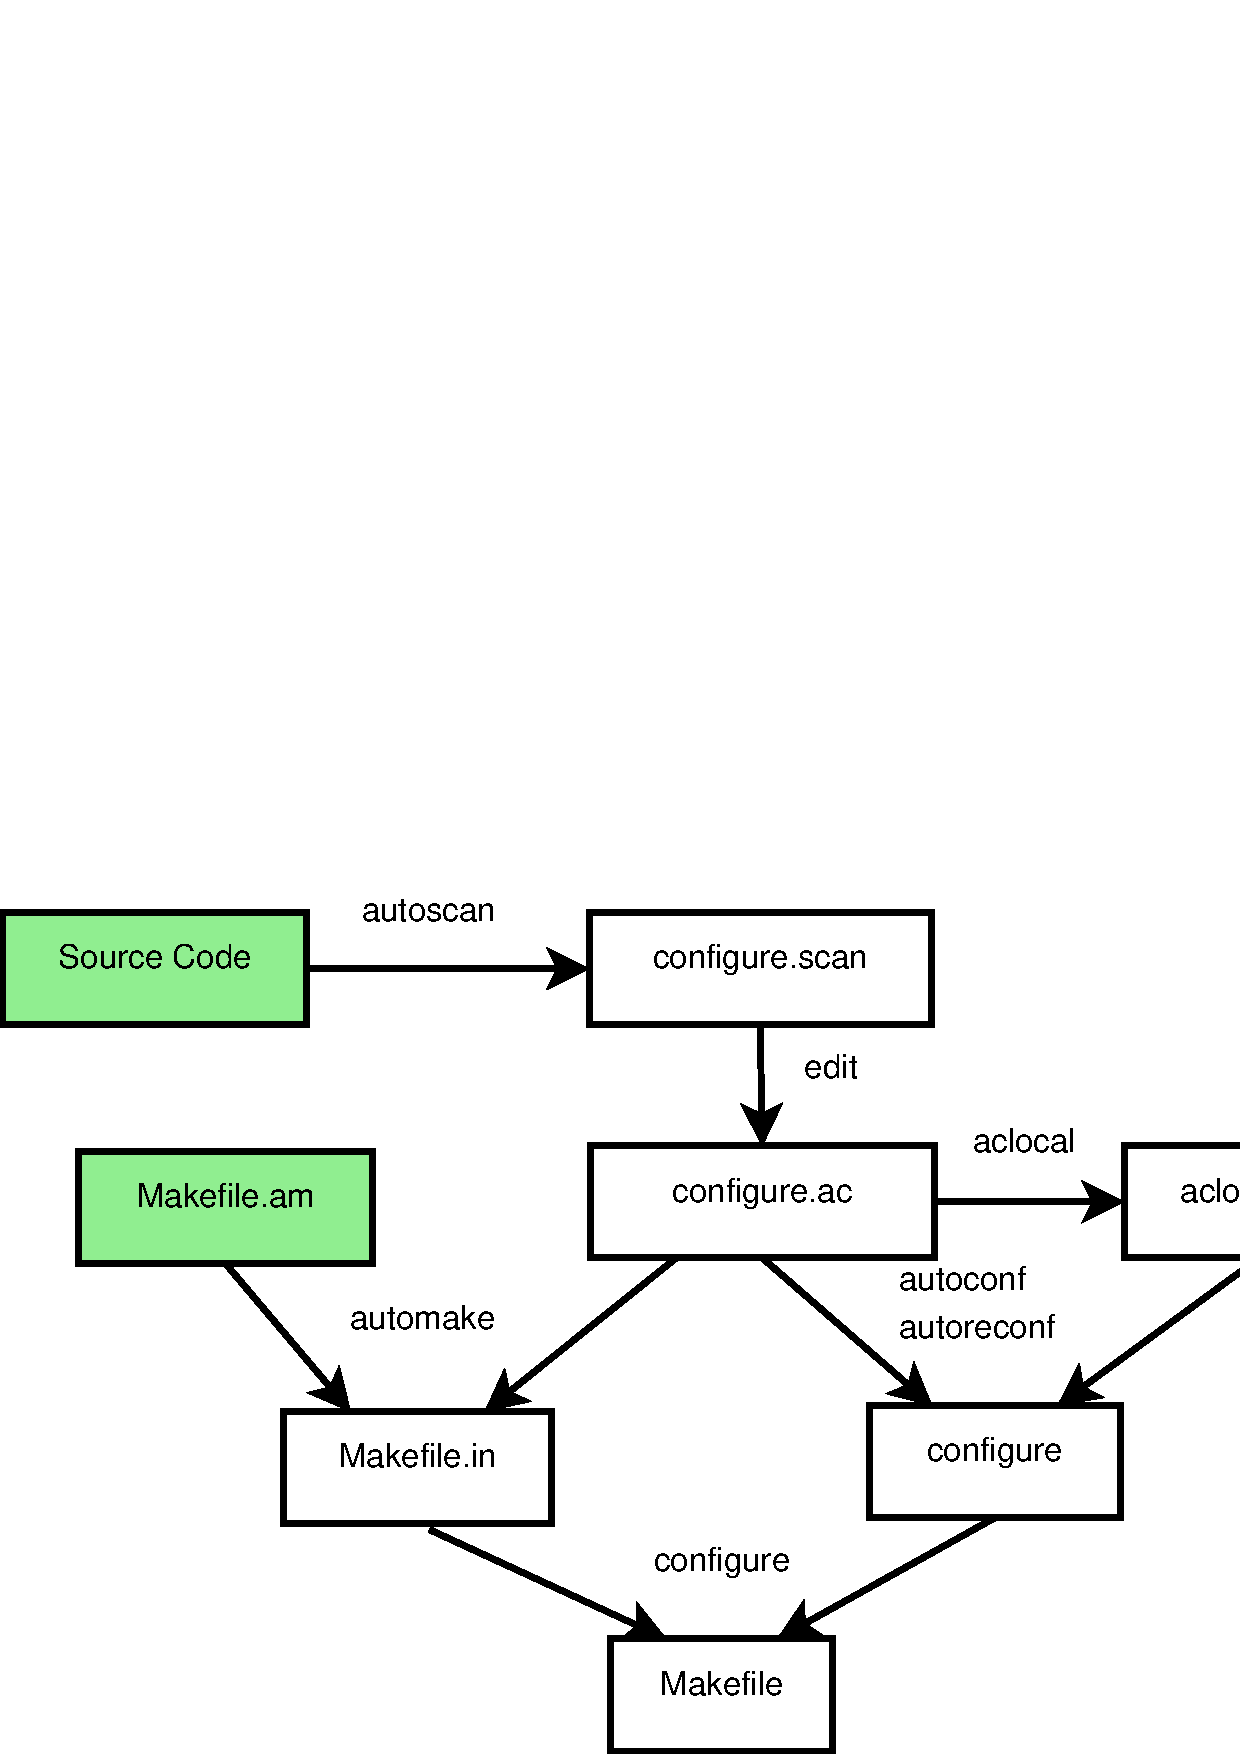
\includegraphics[width=0.8\hsize]{auto.pdf}
  
\end{frame}


\begin{frame}[containsverbatim]
  \frametitle{示例}
  一个简单示例, 项目只包含helloworld.c文件 \\

\begin{Verbatim}
int main(int argc, char ** argv)
{
	printf("Hello, Hello world!\n") ;
	return 0 ;
}
\end{Verbatim}
  
\end{frame}

\begin{frame}[containsverbatim]
  \frametitle{示例: configure.ac}

\begin{Verbatim}[fontsize=\footnotesize]
#    -*- Autoconf -*-
# Process this file with autoconf to produce a configure script.
AC_PREREQ(2.59)
AC_INIT(helloworld, 0.1, caodg@sei.pku.edu.cn)
AC_CONFIG_SRCDIR([helloworld.c])
# Checks for programs.
AC_PROG_CC
# Checks for libraries.
# Checks for header files.
# Checks for typedefs, structures, and compiler characteristics.
# Checks for library functions.
AC_OUTPUT(Makefile)
\end{Verbatim}
\end{frame}

\begin{frame}[containsverbatim]
  \frametitle{示例: Makefile.am}

\begin{Verbatim}
AUTOMAKE_OPTIONS=foreign
bin_PROGRAMS=helloworld
helloworld_SOURCES=helloworld.c
\end{Verbatim}
\end{frame}

\end{document}
